\documentclass{article}

\usepackage{amsmath, amsthm, amssymb}
\usepackage{booktabs}
\usepackage{tikz}
\usepackage{enumitem}
\usepackage{amssymb}
\usepackage{stmaryrd}

% Define a custom chapter counter (manually update this for each chapter)
\newcounter{chapternumber}
\setcounter{chapternumber}{1}  % Set this to the current chapter number

% Define theorem-like environments
\newtheorem{theorem}{Theorem}[section]
\newtheorem{lemma}[theorem]{Lemma}
\theoremstyle{definition}
\newtheorem{definition}[theorem]{Definition}

% Define a problem environment and an exercise environment with numbering tied to section
\newtheorem{problem}{Problem}[section]
\newtheorem{exercise}{Exercise}[section]

% Customize the printed numbers to include our custom chapter counter
\renewcommand{\theproblem}{\arabic{chapternumber}.\thesection.\arabic{problem}}
\renewcommand{\theexercise}{\arabic{chapternumber}.\thesection.\arabic{exercise}}

\begin{document}

\section{Exercises}  % This is Section 1

\begin{exercise}[ex. 9]
    \[
    \begin{aligned}
        |S| &= 25 \\
        |A| &= 40 \\
        |S\cap A| &= 10\\
        |S\cup A| &= ?
    \end{aligned}
\]
\end{exercise}
\begin{proof}[Solution]
\[
    \begin{aligned}
        |S| &= 25 \\
        |A| &= 40 \\
        |S\cap A| &= 10\\
        |S\cup A| &= |S| + |A| - |S\cap A| = 25 + 40 - 10\\
        |S\cup A| &= 55
    \end{aligned}
\]
\end{proof}



\begin{exercise}[ex. 10]
    \[
    \begin{aligned}
        |BUS| &= 30 \\
        |TRAIN| &= 35 \\
        |AUTO| &= 100 \\
        |BUS \cap TRAIN| &= 15 \\
        |BUS \cap AUTO| &= 15 \\
        |TRAIN \cap AUTO| &= 20\\
        |BUS \cap TRAIN \cap AUTO| &= 5 \\
        |BUS \cup TRAIN \cup AUTO| &= ?
    \end{aligned}
\]
\end{exercise}
\begin{proof}[Solution]
\[
    \begin{aligned}
        |BUS \cup TRAIN \cup AUTO| &= |BUS| + |TRAIN| + |AUTO| \\
                                    &- |BUS \cap TRAIN| - |BUS \cap AUTO| - |TRAIN \cap AUTO| \\
                                    &+ |BUS \cap TRAIN \cap AUTO| \\
                                    &= 30 + 35 + 100 - 15 - 15 -20 + 5 \\
                                    &= 120
    \end{aligned}
\]
\end{proof}


\section{Problems}  % This is Section 2

\begin{problem}
\[
    \begin{aligned}
        U &= \{a, b, c, d, e, f, g, h, k\}\\
        A &= \{a, b, c, g\}\\
        B &= \{d, e, f, g\}\\
        C &= \{a, c, f\}\\
        D &= \{f, h, k\}
    \end{aligned}
\]
    \begin{enumerate}[label=(\alph*)]
        Compute

        \item \(A \cup B\) = \{a, b, c, d, e, f, g\}
        \item \(B \cup C\) = \{a, c, d, e, f, g\}
        \item \(A \cap C\) = \{a, c\}
        \item \(B \cap D\) = \{f\}
        \item \((A\cup B)-C\) = \{b, d, e, g\}
        \item \(A-B\) = \{a, b, c\}
        \item \(\overline{A}\) = \{d, e, f, h, k\}
        \item \(A \oplus B\) = \{a, b, c\} $\cup$ \{d, e, f\} = \{a, b, c, d, e, f\}
        \item \(A \oplus C\) = \{b, g\} $\cup$ \{f\} = \{b, g, f\}
        \item \((A\cap B)-C\) = \{g\} - \{a, c, f\} = \{g\}
    \end{enumerate}
\end{problem}


\begin{problem}
\[
    \begin{aligned}
        U &= \{a, b, c, d, e, f, g, h, k\}\\
        A &= \{a, b, c, g\}\\
        B &= \{d, e, f, g\}\\
        C &= \{a, c, f\}\\
        D &= \{f, h, k\}
    \end{aligned}
\]
    \begin{enumerate}[label=(\alph*)]
        Compute

        \item \(A \cup D\) = \{a, b, c , f, g, h, k\}
        \item \(B \cup D\) = \{d, e, f, g, h, k\}
        \item \(C \cap D\) = \{f\}
        \item \(A \cap D\) = $\varnothing$
        \item \((A \cup B) - (C \cup B)\) = \{a, b, c, d, e, f, g\} - \{a, c, d, e, f, g\} = \{b\}
        \item \(B - C\) = \{d, e, g\}
        \item \(\overline{B}\) = \{a, b, c, h, k\}
        \item \(C - B\) = \{a, c\}
        \item \(C \oplus D\) = \{a, c\} $\cup$ \{h, k\} = \{a, c, h, k\}
        \item \((A \cap B) - (B \cap D)\) = \{g\} - \{f\} = \{g\}
    \end{enumerate}
\end{problem}


\begin{problem}
\[
    \begin{aligned}
        U &= \{a, b, c, d, e, f, g, h, k\}\\
        A &= \{a, b, c, g\}\\
        B &= \{d, e, f, g\}\\
        C &= \{a, c, f\}\\
        D &= \{f, h, k\}
    \end{aligned}
\]
    \begin{enumerate}[label=(\alph*)]
        Compute

        \item \(A \cup B \cup C\) = \{a, b, c, d, e, f, g\}
        \item \(A \cap B \cap C\) = $\varnothing$
        \item \(A \cap (B \cup C)\) = $(A \cap B) \cup (A \cap C)$ = \{g\} $\cup$ \{a, c\} = \{a, c, g\}
        \item \((A \cup B) \cap C\) = $(C \cap A) \cup (C \cap B)$ = \{a, c\} $\cup$ \{f\} = \{a, c, f\}
        \item \(\overline{A \cup B}\) = \{d, e, f, h, k\} $\cap$ \{a, b, c, h, k\} = \{h, k\}
        \item \(\overline{A \cap B}\) = \{d, e, f, h, k\} $\cup$ \{a, b, c, h, k\} = \{a, b, c, d, e, f, h, k\}
    \end{enumerate}
\end{problem}


\begin{problem}
\[
    \begin{aligned}
        U &= \{a, b, c, d, e, f, g, h, k\}\\
        A &= \{a, b, c, g\}\\
        B &= \{d, e, f, g\}\\
        C &= \{a, c, f\}\\
        D &= \{f, h, k\}
    \end{aligned}
\]
    \begin{enumerate}[label=(\alph*)]
        Compute

        \item \(A \cup \varnothing\) = A
        \item \(A \cup U\) = U
        \item \(B \cup B\) = B
        \item \(C \cap \varnothing\) = $\varnothing$
        \item \(\overline{C \cup D}\) = \{b, d, e, g, h, k\} $\cap$ \{a, b, c, d, e, g\} = \{b, d, e, g\}
        \item \(\overline{C \cap D}\) = \{b, d, e, g, h, k\} $\cup$ \{a, b, c, d, e, g\} = \{a, b, c, d, e, g, h, k\}

    \end{enumerate}
\end{problem}



\begin{problem}
\[
    \begin{aligned}
        U &= \{1, 2, 3, 4, 5, 6, 7, 8, 9\}\\
        A &= \{1, 2, 4, 6, 8\}\\
        B &= \{2, 4, 5, 9\}\\
        C &= \{x \mid x \in Z^+\ \land x^2 \leq 16\}=\{1, 2, 3, 4\}\\
        D &= \{7, 8\}
    \end{aligned}
\]
    \begin{enumerate}[label=(\alph*)]
        Compute

        \item \(A \cup B\) = \{1, 2, 4, 5, 6, 8, 9\}
        \item \(A \cup C\) = \{1, 2, 3, 4, 6, 8\}
        \item \(A \cup D\) = \{1, 2, 4, 6, 7, 8\}
        \item \(B \cup C\) = \{1, 2, 3, 4, 5, 9\}
        \item \(A \cap C\) = \{1, 2, 4\}
        \item \(A \cap D\) = \{8\}
        \item \(B \cap C\) = \{2, 4\}
        \item \(C \cap D\) = $\varnothing$
    \end{enumerate}
\end{problem}


\begin{problem}
\[
    \begin{aligned}
        U &= \{1, 2, 3, 4, 5, 6, 7, 8, 9\}\\
        A &= \{1, 2, 4, 6, 8\}\\
        B &= \{2, 4, 5, 9\}\\
        C &= \{x \mid x \in Z^+\ \land x^2 \leq 16\}=\{1, 2, 3, 4\}\\
        D &= \{7, 8\}
    \end{aligned}
\]
    \begin{enumerate}[label=(\alph*)]
        Compute

        \item \(A - B\) = \{1, 6, 8\}
        \item \(B - A\) = \{5, 9\}
        \item \(C - D\) = \{1, 2, 3, 4\}
        \item \(\overline{C}\) = \{5, 6, 7, 8, 9\}
        \item \(\overline{A}\) = \{3, 5, 7, 9\}
        \item \(A \varoplus B\) = \{1, 6, 8\} $\cup$ \{5, 9\} = \{1, 5, 6, 8, 9\}
        \item \(C \varoplus D\) = \{1, 2, 3, 4, 7, 8\}
        \item \(B \varoplus C\) = \{1, 3, 5, 9\}
    \end{enumerate}
\end{problem}


\begin{problem}
\[
    \begin{aligned}
        U &= \{1, 2, 3, 4, 5, 6, 7, 8, 9\}\\
        A &= \{1, 2, 4, 6, 8\}\\
        B &= \{2, 4, 5, 9\}\\
        C &= \{x \mid x \in Z^+\ \land x^2 \leq 16\}=\{1, 2, 3, 4\}\\
        D &= \{7, 8\}
    \end{aligned}
\]
    \begin{enumerate}[label=(\alph*)]
        Compute

        \item \(A \cup B \cup C\) = \{1, 2, 3, 4, 5, 6, 8, 9\}
        \item \(A \cap B \cap C\) = \{2, 4\}
        \item \(A \cap (B \cup C)\) = \{1, 2, 4\}
        \item \((A \cup B) \cap D\) = \{8\}
        \item \(\overline{A \cup B}\) = \{3, 5, 7, 9\} $\cap$ \{1, 3, 6, 7, 8\} = \{3, 7\}
        \item \(\overline{A \cap B}\) = \{3, 5, 7, 9\} $\cup$ \{1, 3, 6, 7, 8\} = \{1, 3, 5, 6, 7, 8, 9\}
    \end{enumerate}
\end{problem}


\begin{problem}
\[
    \begin{aligned}
        U &= \{1, 2, 3, 4, 5, 6, 7, 8, 9\}\\
        A &= \{1, 2, 4, 6, 8\}\\
        B &= \{2, 4, 5, 9\}\\
        C &= \{x \mid x \in Z^+\ \land x^2 \leq 16\}=\{1, 2, 3, 4\}\\
        D &= \{7, 8\}
    \end{aligned}
\]
    \begin{enumerate}[label=(\alph*)]
        Compute

        \item \(B \cup C \cup D\) = \{1, 2, 3, 4, 5, 7, 8, 9\}
        \item \(B \cap C \cap D\) = $\varnothing$
        \item \(A \cup A\) = \{1, 2, 4, 6, 8\}
        \item \(A \cap \overline{A}\) = $\varnothing$
        \item \(A \cup \overline{A}\) = \{1, 2, 3, 4, 5, 6, 7, 8, 9\}
        \item \(A \cap (\overline{C} \cup D)\) = \{6, 8\} $\cup$ \{8\} = \{6, 8\}

    \end{enumerate}
\end{problem}


\begin{problem}
\[
    \begin{aligned}
        U &= \{a, b, c, d, e, f, g, h\}\\
        A &= \{a, c, f, g\}\\
        B &= \{a, e\}\\
        C &= \{b, h\}
    \end{aligned}
\]
    \begin{enumerate}[label=(\alph*)]
        Compute

        \item \(\overline{A}\) = \{b, d, e, h\}
        \item \(\overline{B}\) = \{b, c, d, f, g, h\}
        \item \(\overline{A \cup B}\) = \{b, d, h\}
        \item \(\overline{A \cap B}\) = \{b, c, d, e, f, g, h\}
        \item \(\overline{U}\) = $\varnothing$
        \item \(A - B\) = \{c, f, g\}

    \end{enumerate}
\end{problem}


\begin{problem}
\[
    \begin{aligned}
        U &= \{a, b, c, d, e, f, g, h\}\\
        A &= \{a, c, f, g\}\\
        B &= \{a, e\}\\
        C &= \{b, h\}
    \end{aligned}
\]
    \begin{enumerate}[label=(\alph*)]
        Compute

        \item \(\overline{A} \cap \overline{B}\) = \{b, d, e, h\} $\cap$ \{b, c, d, f, g, h\} = \{b, d, h\}
        \item \(\overline{B} \cup \overline{C}\) = \{b, c, d, f, g, h\} $\cup$ \{a, c, d, e, f, g\} = \{a, b, c, d, e
        , f, g, h\}
        \item \(\overline{A \cup A}\) = $\overline{A}$ = \{b, d, e, h\}
        \item \(\overline{C \cap C}\) = $\overline{C}$ = \{a, c, d, e, f, g\}
        \item \(A \oplus B\) = \{c, e, f, g\}
        \item \(B \oplus C\) = \{a, e, b, h\}

    \end{enumerate}
\end{problem}

\begin{problem}
\[
    \begin{aligned}
        U &= R\\
        A &= \{x \mid x \text{ is a solution to } x^2 -1 = 0\} = \{-1, 1\}\\
        B &= \{-1, 4\}\\
    \end{aligned}
\]
    \begin{enumerate}[label=(\alph*)]
        Compute

        \item \(\overline{A}\) = $\{x \mid x \in (-\infty, -1) \lor (-1, 1) \lor x \in (1, \infty)\}$
        \item \(\overline{B}\) = $\{x \mid x \in (-\infty, -1) \lor x \in (-1, 4) \lor x \in (4, \infty)\}$
        \item \(\overline{A \cup B}\) = $\{x \mid x \in (-\infty, -1) \lor (-1, 1) \lor (1, 4) \lor x \in (4, \infty)\}$
        \item \(\overline{A \cap B}\) = $\{x \mid x \in (-\infty, -1) \lor (-1, \infty)\}$

    \end{enumerate}
\end{problem}

\begin{problem}
\[

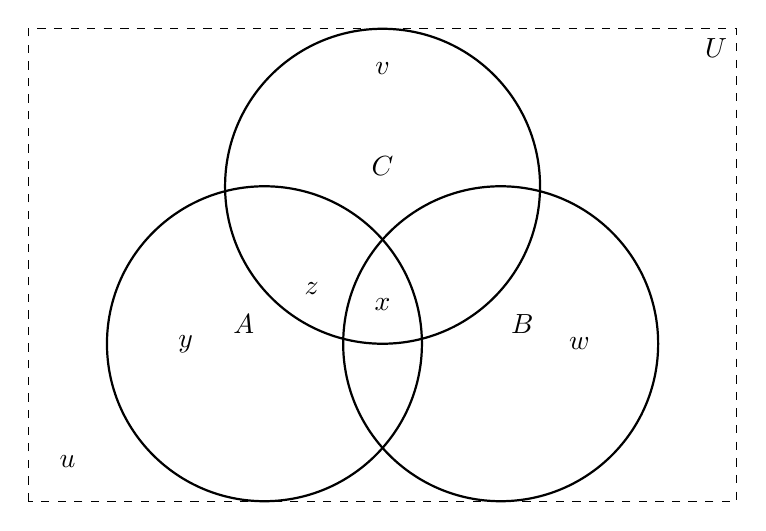
\begin{tikzpicture}[scale=1.0]

  % Draw the universal set as a dashed rectangle
  \draw[dashed] (-3,-2) rectangle (6,4);
  \node[anchor=north east] at (6,4) {$U$};

  % Draw circles for sets A, B, and C
  \draw[thick] (0,0) circle (2) node[above left] {$A$};
  \draw[thick] (3,0) circle (2) node[above right] {$B$};
  \draw[thick] (1.5,2) circle (2) node[above] {$C$};

  % Place elements in the regions
  \node at (-1,0) {$y$};       % In A only
  \node at (4,0) {$w$};        % In B only
  \node at (1.5,3.5) {$v$};     % In C only
  \node at (1.5,0.5) {$x$};     % In A ∩ B ∩ C (central intersection; moved lower)
  \node at (0.6,0.7) {$z$};       % In A ∩ B (but outside C; moved left and up)
  \node at (-2.5,-1.5) {$u$};   % In U, outside all three sets

\end{tikzpicture}
\]
    \begin{enumerate}[label=(\alph*)]
        Compute

        \item \(y \in A \cap B\) = False: y $\notin$ B
        \item \(x \in B \cup C\) = True: x $\in$ B $\land$ x $\in$ C
        \item \(w \in B \cap C\) = False: w $\notin$ C
        \item \(u \notin C\) = True: u $\in \overline{A \cup B \cup C}$

    \end{enumerate}
\end{problem}

\begin{problem}
\[

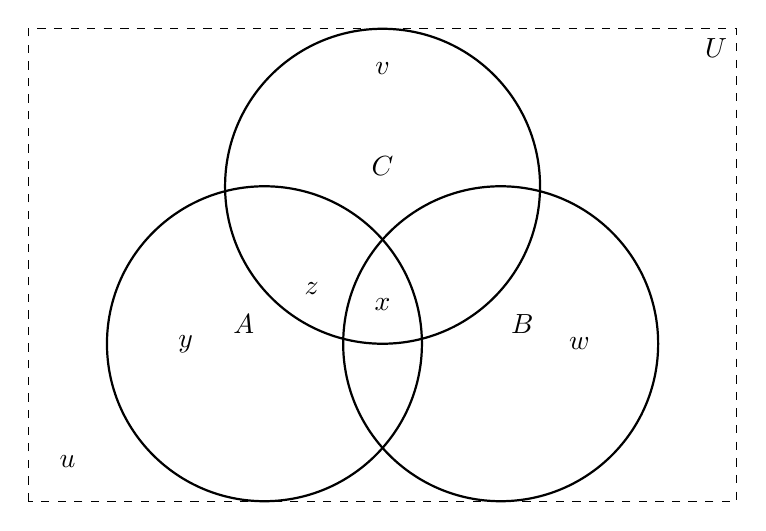
\begin{tikzpicture}[scale=1.0]

  % Draw the universal set as a dashed rectangle
  \draw[dashed] (-3,-2) rectangle (6,4);
  \node[anchor=north east] at (6,4) {$U$};

  % Draw circles for sets A, B, and C
  \draw[thick] (0,0) circle (2) node[above left] {$A$};
  \draw[thick] (3,0) circle (2) node[above right] {$B$};
  \draw[thick] (1.5,2) circle (2) node[above] {$C$};

  % Place elements in the regions
  \node at (-1,0) {$y$};       % In A only
  \node at (4,0) {$w$};        % In B only
  \node at (1.5,3.5) {$v$};     % In C only
  \node at (1.5,0.5) {$x$};     % In A ∩ B ∩ C (central intersection; moved lower)
  \node at (0.6,0.7) {$z$};       % In A ∩ B (but outside C; moved left and up)
  \node at (-2.5,-1.5) {$u$};   % In U, outside all three sets

\end{tikzpicture}
\]
    \begin{enumerate}[label=(\alph*)]
        Compute

        \item \(x \in A \cap B \cap C\) = True: x $\in$ A $\land$ x $\in$ B $\land$ x $\in$ C
        \item \(y \in A \cup B \cup C\) = True: y $\in$ A
        \item \(z \in A \cap C\) = True: z $\in$ A $\land$ z $\in$ C
        \item \(v \in B \cap C\) = False: v $\in$ C $\land$ v $\notin$ B

    \end{enumerate}
\end{problem}











\begin{problem}
\[

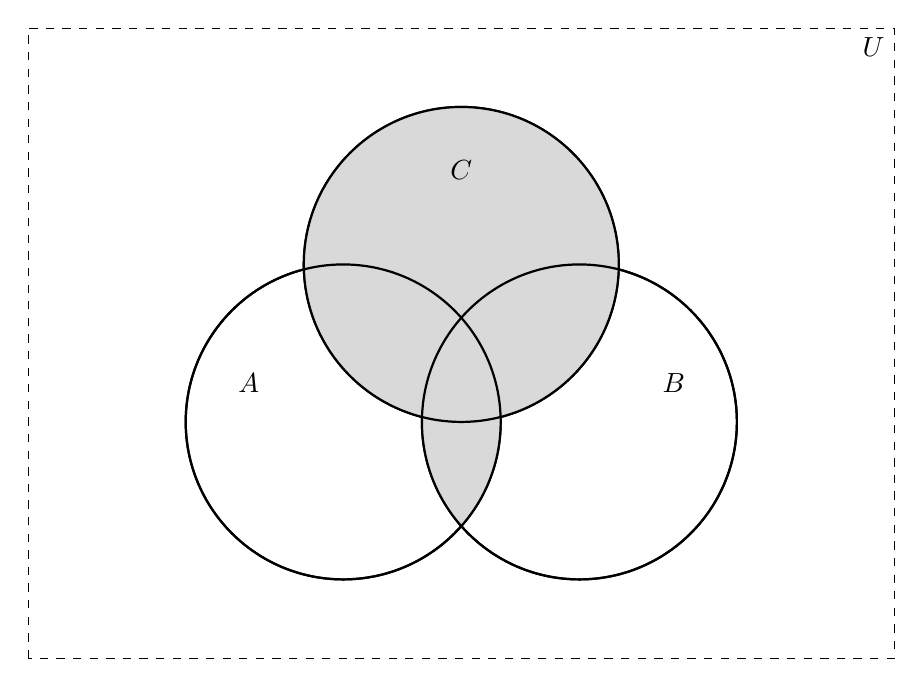
\begin{tikzpicture}[scale=1.0]

  % Draw the universal set as a dashed rectangle
  \draw[dashed] (-4,-3) rectangle (7,5);
  \node[anchor=north east] at (7,5) {$U$};

  % Define radius for circles
  \def\r{2}

  % Draw circles for sets A, B, and C
  \draw[thick] (0,0) circle (\r);
  \draw[thick] (3,0) circle (\r);
  \draw[thick] (1.5,2) circle (\r);

%  % Place labels for the sets
%  \node at (-1.2,1.5) {$A$};
%  \node at (4.2,1.5) {$B$};
%  \node at (1.5,3.2) {$C$};

  % Shade entire circle C
  \begin{scope}
    \clip (1.5,2) circle (\r);
    \fill[gray!30] (-4,-3) rectangle (7,5);
  \end{scope}

  % Shade the region A ∩ B (this may extend outside C)
  \begin{scope}
    \clip (0,0) circle (\r);
    \clip (3,0) circle (\r);
    \fill[gray!30] (-4,-3) rectangle (7,5);
  \end{scope}

  % Redraw circles (so that outlines and labels remain visible)
  \draw[thick] (0,0) circle (\r);
  \draw[thick] (3,0) circle (\r);
  \draw[thick] (1.5,2) circle (\r);

  % Optionally, redraw the labels on top
  \node at (-1.2,0.5) {$A$};
  \node at (4.2,0.5) {$B$};
  \node at (1.5,3.2) {$C$};

\end{tikzpicture}
\]
    \begin{enumerate}[label=(\alph*)]
        Describe shaded region

        $$ (A \cap B) \cup C $$

    \end{enumerate}
\end{problem}

%\begin{proof}[Solution.]
%\begin{enumerate}[label=(\alph*),leftmargin=*]
%%    \newline
%%    \item \( A \cup B = \{a, b, c, d, e, f, g\} \).
%%    \item \( B \cup C = \{a, c, d, e, f, g\} \).
%%    \item \( A \cap C = \{a, c\} \).
%%    \item \( B \cap D = \{f\} \).
%%    \item \( (A\cup B)-C = \{b, d, e, g\} \).
%%    \item \( A - B = \{a, b, c\} \).
%%    \item \( \overline{A} = \{d, e, f, h, k\} \).
%%    \item \( A \oplus B = (A - B) \cup (B - A) = \{a,b,c,d,e,f\} \).
%%    \item \( A \oplus C = (A - C) \cup (C - A) = \{b,g,f\} \).
%%    \item \( (A \cap B) - C = \{g\} \).
%\end{enumerate}
%\end{proof}

\end{document}
